\section{Mariages, couplages et couvertures}
\subsection{Couplage}
\index{couplage}
\begin{mydef}
  Un \emph{couplage} dans un graphe est un ensemble $M$ d’arêtes tel que $M$ ne contient pas de boucles et deux arêtes de $M$ n’ont jamais d’extrêmité en commun.
\end{mydef}

\index{couplage!couplage maximum}
\begin{mydef}
  Un \emph{couplage maximum} est un couplage dont le nombre d’arêtes est maximal.
\end{mydef}

\index{couplage!couplage parfait}
\begin{mydef}
  Un \emph{couplage parfait} est un couplage qui est incident à tous les noeuds.
\end{mydef}

\begin{myrem}
  Un couplage parfait, s’il existe, est maximum.
\end{myrem}

\index{chemin!chemin M-alterné}
\begin{mydef}
  Pour un couplage $M$, un \emph{chemin M-alterné} est un chemin qui passe alternativement par une arête de $M$ et par une arête hors de $M$.
\end{mydef}

\index{chemin!chemin M-augmenté}
\begin{mydef}
  Un \emph{chemin M-augmenté} est un chemin M-alterné dont les noeuds d’origine et de destination ne sont pas incident à une arête de $M$.
\end{mydef}

\begin{mytheo} [Berge]
  Un couplage $M$ est maximum si et seulement s’il n’y a pas de chemin $M$-augmenté.
  \begin{proof}
     Preuve:
$ \Longrightarrow $ Soit le couplage $M$, représenté en bleu sur la figure ci-dessous, et un chemin $M$-augmenté en vert que nous noterons $P$.

\begin{center}
    \begin{tikzpicture}[scale=1]
      \SetGraphUnit{1}
      \SetVertexNoLabel
      \Vertex{A}
      \EA(A){B}
      \EA(B){C}
      \SO(C){D}
      \WE(D){E}
      \EA(C){F}
      \EA(F){G}
      \SO(G){H}
      \Edges(C,D)
      \SetUpEdge[color=green]
      \Edges(A,B)
      \Edges(C,F)
      \Edges(G,H)
      \tikzset{EdgeStyle/.style={color=blue,thick,double=green,double distance = 1.2pt}}
      \Edges(F,G)
      \Edges(B,C)
      \SetUpEdge[color=blue]
      \Edges(D,E)
    \end{tikzpicture}
\end{center}

     On construit le couplage $ M' = M \Delta P$ où $\Delta$ indique une différence symétrique entre $M$ et $P$ ($ M \Delta P = ( M \backslash P) \cup ( P \backslash M)$ ). Ce nouveau couplage est représenté en rouge.
     $ |M'| = |M| + 1 $. On voit bien que M n'est pas maximal.

\begin{center}
    \begin{tikzpicture}[scale=1]
      \SetGraphUnit{1}
      \SetVertexNoLabel
      \Vertex{A}
      \EA(A){B}
      \EA(B){C}
      \SO(C){D}
      \WE(D){E}
      \EA(C){F}
      \EA(F){G}
      \SO(G){H}
      \Edges(C,D)
      \Edges(F,G)
      \Edges(B,C)
      \SetUpEdge[color=red]
      \Edges(G,H)
      \Edges(C,F)
      \Edges(A,B)
      \Edges(D,E)
    \end{tikzpicture}
\end{center}

     $\Longleftarrow$ Soit $M'$ le couplage maximum représenté ci-dessous tel que $ |M'| > |M| $.

\begin{center}
\begin{tikzpicture}
\SetVertexNoLabel
\GraphInit[vstyle=Normal]
\SetGraphUnit{1}
\begin{scope}[rotate=90]
\Vertices{circle}{A,B,C,D}
\end{scope}
\begin{scope}[rotate=90,shift={(0,-3.5)}]
\Vertices{circle}{E,F,G,H}
\end{scope}
\begin{scope}[rotate=90,shift={(0,3.5)}]
\Vertices{circle}{I,J,K,L}
\end{scope}
\EA(H){M}
\Edges(F,G)
%\Edges(I,A)
\Edges(J,L,B,A,C,D,F,H,G,C)
\SetUpEdge[color=red]
\Edges(B,C)
\Edges(F,E)
\Edges(H,M)
\Edges(J,I)
\Edges(K,L)
\SetUpEdge[color=blue]
\Edges(J,K)
\Edges(I,L)
\Edges(E,H)
\tikzset{EdgeStyle/.style={color=blue,thick,double=red,double distance = 1.2pt}}
\Edges(A,D)
\end{tikzpicture}
\end{center}

     Regardons $ M \Delta M'$.

\begin{center}
\begin{tikzpicture}
\SetVertexNoLabel
\GraphInit[vstyle=Normal]
\SetGraphUnit{1}
\begin{scope}[rotate=90]
\Vertices{circle}{A,B,C,D}
\end{scope}
\begin{scope}[rotate=90,shift={(0,-3.5)}]
\Vertices{circle}{E,F,G,H}
\end{scope}
\begin{scope}[rotate=90,shift={(0,3.5)}]
\Vertices{circle}{I,J,K,L}
\end{scope}
\EA(H){M}
\SetUpEdge[color=red]
\Edges(B,C)
\Edges(F,E)
\Edges(H,M)
\Edges(J,I)
\Edges(K,L)
\SetUpEdge[color=blue]
\Edges(J,K)
\Edges(I,L)
\Edges(E,H)
\end{tikzpicture}
\end{center}

     On observe que les noeuds dans $ M \Delta M'$ dont de degrés $0,1$ ou $2$. Les noeuds de degrés $2$ ont une arête dans $M$ et une arête dans $M'$. $\Rightarrow$ $ M \Delta M'$ est une union de noeuds isolés, chemins et cycles. Or, dans un cycle de longueur paire, il y a autant d'arêtes dans $M$ que dans $M'$. Comme  $ |M'| > |M| $, il faut qu'il existe un chemin de longueur impaire qui commence et termine par une arête de $M'$. On voit facilement que ce chemin est un chemin $M$-augmenté.

  \end{proof}
\end{mytheo}
\begin{myexem}
  Exemple \addTODO
\end{myexem}

\begin{mytheo} [Théorème du mariage ou de Hall]
  Un graphe biparti avec bipartition $(X , Y)$ possède un couplage incident à tous les noeuds de $X$
  si et seulement si pour tout ensemble $S \subseteq X$, le nombre de voisins de $S$ est au moins $|S|$.
  \begin{proof}
    Montrons les deux sens, l'un après l'autre.
    \begin{itemize}
      \item[$\Longrightarrow$]
        Un couplage $M$ incident à tout $x \in X$ crée une fonction injective
        $f_M : x \to Y: x \mapsto y$ où $y$ est le noeud associé à $x$ dans le couplage $M$.
        On a $\forall S \subseteq X$, $f_M(S) \subseteq \voisin(S)$.
        Dès lors, $|\voisin(S)| \geq |f_M(S)| = |S|$.
      \item[$\Longleftarrow$]
        On veut montrer qu'il n'existe pas de couplage incident à tout $X$
        et donc qu'il existe un $S \subseteq X : |\voisin(S)| < |S|$.

        Soit $M^*$ le couplage maximal et $u \in X$ non incident à $M^*$.
        Prenons les chemins $M^*$ alternés partant de $u$:
        Soit $Z$ l'ensemble des noeuds ainsi rencontrés.
        $S = X \cap Z$, $T = Y \cap Z$.

        On remarque que
        \begin{itemize}
          \item $\voisin(S) = T$ (par construction);
          \item	$M^*$ est incident à tout $T$ (sinon on aurait un chemin $M$-augmenté car un chemin alterné qui part de $u$ et qui arrive dans $T$ peut toujours poursuivre par une arête de $M^*$);
          \item $M^*$ est incident à tout $S\backslash\lbrace u\rbrace$ par construction;
          \item $M^*$ crée une bijection entre $S\backslash\lbrace u\rbrace$ et $T$
            (car $f_{M^*} (S\setminus \lbrace u\rbrace) \subseteq T$ et
            $f_{M^*}(T) \subseteq S\setminus\lbrace u\rbrace$.
        \end{itemize}
        On a dès lors $\voisin(S) = T$ d'où $|\voisin(S)| = |S| - 1 < |S|$.

        \begin{center}
          \begin{tikzpicture}
            \SetVertexNoLabel
            \tikzset{
              decoration={brace},
              tuborg/.style={decorate},
              tubnoderight/.style={midway, right=2pt},
              tubnodeleft/.style={midway, left=2pt},
            }
            \GraphInit[vstyle=Normal]
            \SetGraphUnit{1.5}
            \Vertex[NoLabel=false,L=$u$]{u}
            \SO(u){A1}
            \SO(A1){B1}
            \SO(B1){C1}
            \SO(C1){D1}
            %\begin{scope}[shift={(0,1.5)}]
            \EA(A1){A2}
            \SO(A2){B2}
            \SO(B2){C2}
            \SO(C2){D2}
            \SO(D2){E2}
            %\end{scope}
            \Edges(u,A2,C1)
            \Edges(C2,A1,B2)
            \Edges(D1,E2)
            \SetUpEdge[color=green]
            \Edges(A1,A2)
            \Edges(B1,B2)
            \Edges(C1,C2)
            \Edges(D1,D2)

            \draw[tuborg, decoration={brace}] let \p1=(u.north), \p2=(C1.south) in ($(-0.5, \y2)$) -- ($(-0.5, \y1)$) node[tubnodeleft] {$S$};
            \draw[tuborg, decoration={brace}] let \p1=(D1.north), \p2=(D1.south) in ($(-0.5, \y2)$) -- ($(-0.5, \y1)$) node[tubnodeleft] {$X\setminus S$};
            \draw[tuborg, decoration={brace}] let \p1=(A2.north), \p2=(C2.south) in ($(2.0, \y1)$) -- ($(2.0, \y2)$) node[tubnoderight] {$T$};
            \draw[tuborg, decoration={brace}] let \p1=(D2.north), \p2=(E2.south) in ($(2.0, \y1)$) -- ($(2.0, \y2)$) node[tubnoderight] {$Y\setminus T$};
          \end{tikzpicture}
        \end{center}
    \end{itemize}
  \end{proof}
\end{mytheo}
\begin{myexem}
  Exemple \addTODO
\end{myexem}

\begin{myrem}
  Un graphe est k-régulier si tous les noeuds sont de degré $k$.
\end{myrem}

\begin{mycorr}[du théorème de Hall]
  Tout graphe biparti k-régulier (pour $k > 0$) possède un couplage parfait.
  \begin{proof}
  Soit $(X,Y)$ la bipartition, le nombre d'arêtes = $\frac{(|X| + |Y|) k}{2} = |X| k = |Y| k$ avec ($k$ le dégré de couplage). $\Rightarrow |X| = |Y|$

  Soit $S \subseteq X$:
  \begin{itemize}
   \item $E_{1} = \lbrace \ arêtes\ incidentes\ à S \rbrace$
   \item $E_{2} = \lbrace \ arêtes\ incidentes\ Voisin(S) \rbrace$
   \end{itemize}

  On remarque:
  \begin{itemize}
  \item $E_{1} \subseteq E_{2}$
  \item $|E_{1}| = |S| k$
  \item $|E_{2}| = |Voisin(S)| k$
  \end{itemize}
  $\Rightarrow |S| \leq |Voisin(S)|$

  Donc le théorème de Hall s'applique car il existe un couplage incident à $X$ et il existe un couplage parfait car $|X|=|Y|$
  \end{proof}
\end{mycorr}

\subsection{Couverture}
\index{couverture de sommets}
\begin{mydef}
  Une \emph{couverture de sommets} d’un graphe est un ensemble de sommets incident à toutes les arêtes.
\end{mydef}

\index{couverture de sommets!minimum}
\begin{mydef}
  Une \emph{couverture de sommets minimum} d’un graphe est une couverture de sommets avec un nombre minimal de sommets.
\end{mydef}

\begin{myrem}
  Si $K$ est une couverture de sommets et $M$ un couplage, alors $|M| \leq |K|$.
\end{myrem}

\begin{myrem}
  Si $K^*$ est une couverture de sommets minimum et $M$ un couplage maximum, alors $|M^*| \leq |K^*|$.
\end{myrem}

\begin{mylem}
  Si $K$ est une couverture de sommets, $M$ un couplage et que $|M| = |K|$, alors $K$ est minimum et $M$ est maximum.
  \begin{proof}
     Preuve: on a, par définition, $|M| \leq |M^*| \leq |k^*| \leq |k|$. par conséquent, si $|M| = |K|$, $|M| = |M^*| = |K^*| = |K|$
  \end{proof}
\end{mylem}

\begin{mytheo} [König]
  Dans un graphe biparti, si $K^*$ est une couverture de sommets minimum et $M^*$ un couplage maximum, alors $|M^*| = |K^*|$.
  \begin{proof} [Démonstration venant du cours de R. Lambiotte et L. Tabourier  (FUNDP)]
    Soit un graphe biparti ($X$,$Y$) et $M^*$ un couplage maximum.
    Soit $U$ les noeuds qui ne sont pas incidents à $M^*$ dans $X$.
    Soit $Z$ l'ensemble des noeuds atteints par tous les chemins $M^*$-alternés partant de $U$.\\
    Soient :
    \begin{enumerate}
      \item $S = Z \cap X$
      \item $T = Z \cap Y$
    \end{enumerate}
    On montre que $V(S) = T$ :
    \begin{center}
      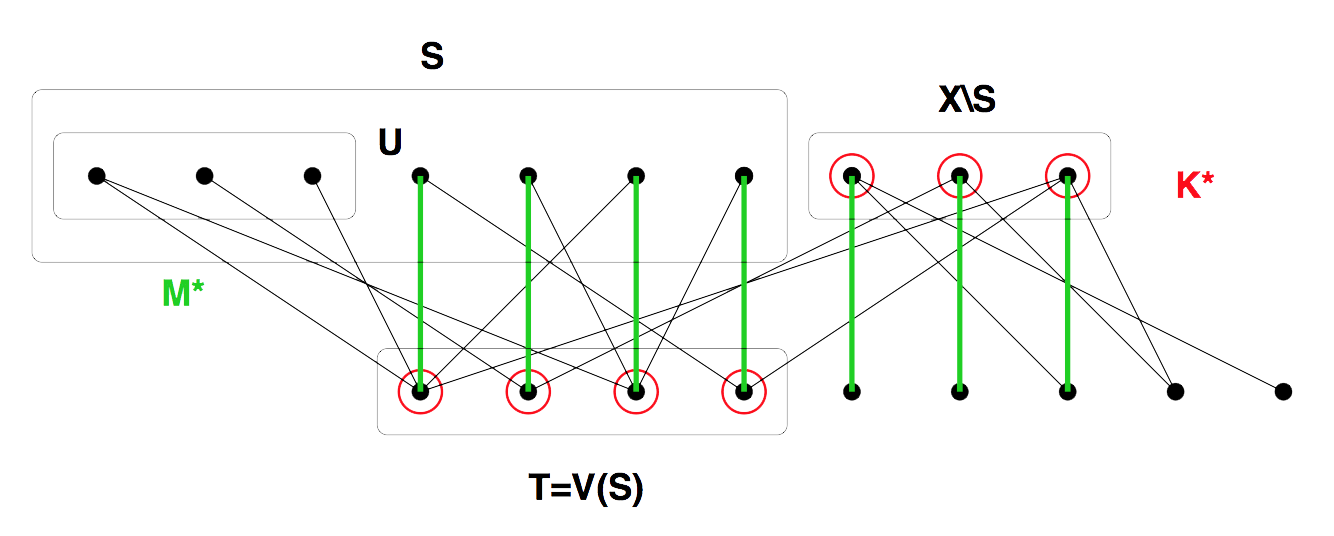
\includegraphics[width=300pt]{../img/konig}
    \end{center}
    Soit $K = T \cup (X \textbackslash S)$, $K$ est une couverture de sommets : toutes les arêtes ont une extrêmité dans $K$ car si ce n'est pas le cas, on a une arête du graphe liant $(Y \textbackslash T)$ à $S$, or $V(S) = T$ (contradictoire). On va montrer que $K$ est une couverture minimale et qu'elle vérifie $|K^*| = |M^*|$.\\
    $|K| = |X \textbackslash S| + |T|$ ($X$ et $Y$ étant disjoints).\\
    Supposons qu'il existe $x \in X \textbackslash S$ tel que $x$ est adjacent par une arête de $M^*$ à un noeud de $T$, dans ce cas $x \in Z$ et donc $x \in S$ (contradictoire). Donc les arêtes de $M^*$ ont une extrémité dans $T$ ou dans $X \textbackslash S$ mais pas dans les deux, donc $|K| = |M^*|$, on a donc trouvé que $K^*$ est une couverture minimum telle que $|K^*| = |M^*|$.\\
    Notons qu'on a pas seulement montré qu'il existe une couverture minimum $K^*$ telle que $|K^*| = |M^*|$, on a aussi vu comment on pouvait la construire connaissant $M^*$.
  \end{proof}
\end{mytheo}

\begin{myexem}[Problème du site de rencontres]
	Nous avons 5 filles et 5 garçons (noeuds) et nous devons en accoupler un maximum en fonction de leurs préférences (arêtes = volonté de s'accoupler). Par conséquent, nous devons réaliser un couplage maximum sur un graphe biparti. Voici le schéma obtenu :
	\begin{center}
	  \begin{tikzpicture}
      \node[vertex] at (-2, 2) (a) {A};
			\node[vertex] at (-1, 2) (b) {B};
			\node[vertex, fill = red] at (0, 2) (c) {C};
			\node[vertex, fill = red] at (1, 2) (d) {D};
			\node[vertex] at (2, 2) (e) {E};
			\node[vertex] at (-2, -2) (f) {a};
			\node[vertex, fill = red] at (-1, -2) (g) {b};
			\node[vertex] at (0, -2) (h) {c};
			\node[vertex, fill = red] at (1, -2) (i) {d};
			\node[vertex] at (2, -2) (j) {e};

      \draw[red] (a) edge node {} (g);
			\draw[] (a) edge node {} (i);
			\draw[] (b) edge node {} (g);
			\draw[] (c) edge node {} (f);
			\draw[] (c) edge node {} (g);
			\draw[red] (c) edge node {} (h);
			\draw[] (c) edge node {} (i);
			\draw[] (c) edge node {} (j);
			\draw[] (d) edge node {} (h);
			\draw[red] (d) edge node {} (j);
			\draw[red] (e) edge node {} (i);
  	\end{tikzpicture}
  \end{center}
On voit que $|M|=|K|$ et, par conséquent (voir en rouge), le couplage est maximum (et la couverture est minimum).
\end{myexem}

\subsection{L'algorithme hongrois}
\index{algorithme!algorithme hongrois}
\begin{myalgo}[Algorithme hongrois venant du cours de R. Lambiotte et L. Tabourier (FUNDP)]
  \noindent
  \begin{enumerate}
    \item Construire un couplage $M$ du graphe biparti tel qu'on ne puisse plus ajouter d'arêtes sans que deux arêtes soient incidentes au même noeud
    \item Soit $U = \{u \in X$ et $u$ non-incident à $M^*\}$, si $U = \o$, le couplage est maximum (arrêt)
    \item $\forall u \in U$, on construit l'ensemble des chemins M-alternés partant de $u$ (étape non-triviale)
      \begin{itemize}
        \item soit aucun de ces chemins n'est M-augmenté, par théorème le couplage est maximum (arrêt)
        \item soit il existe un chemin M-augmenté $u,y_a,x_b,...,x_l,y_m$, et on modifie M selon :\\
        $M \leftarrow M \textbackslash\{(y_a,x_b),...,(y_k,x_l)\} \cup \{(u,ya),(xb,yc),...,(xl,ym)\}$
      \end{itemize}
    \item on itère le procédé jusqu'à avoir un couplage maximum
  \end{enumerate}
\end{myalgo}
\begin{myexem}
  \noindent
  \begin{enumerate}
    \item couplage initial :\\
      \begin{center}
        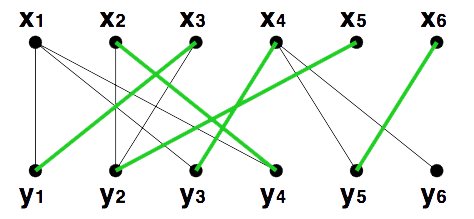
\includegraphics[width=150pt]{../img/hongrois1}
      \end{center}
    \item recherche des chemins alternés :\\
      \begin{center}
        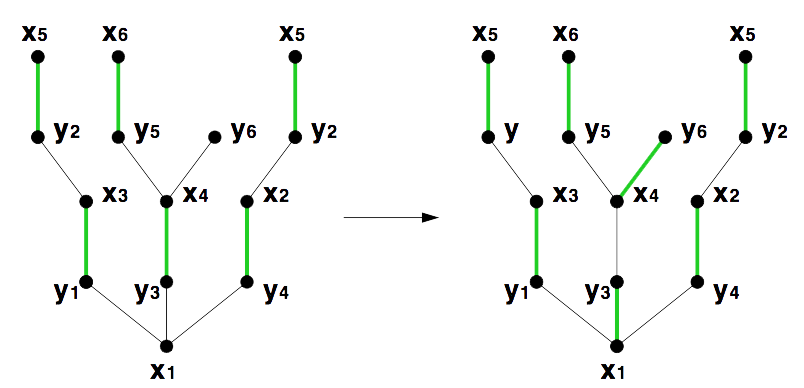
\includegraphics[width=250pt]{../img/hongrois2}
      \end{center}
    \item couplage suivant (et maximum) :\\
      \begin{center}
        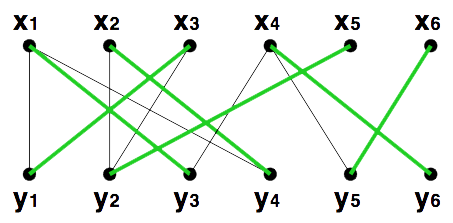
\includegraphics[width=150pt]{../img/hongrois3}
      \end{center}
  \end{enumerate}
\end{myexem}
